% ==============================================================================
% Capítulo 7: Verificação, validação e testes
% ==============================================================================
\chapter{Verificação, validação e testes}
\label{cap:testes}

\begin{instrucao}
\orientacao{O que vai em Verificação, Validação e Testes}
Este capítulo mostra que o sistema funciona e que atende aos requisitos.
Distinga dois aspectos:
\begin{itemize}
  \item \textbf{verificação}: o sistema foi construído corretamente? Testes
        automatizados (unidade, integração, sistema), cobertura, análise
        estática;
  \item \textbf{validação}: o sistema certo foi construído? Avaliação com
        usuários reais, testes de aceitação, medidas de usabilidade.
\end{itemize}
Retome os requisitos funcionais e não funcionais e mostre, para cada um, como
foi verificado e com que resultado. Requisitos não atendidos também devem ser
relatados, com a explicação do motivo.

\textbf{Atenção:} todos os números deste capítulo de exemplo são fictícios.
\end{instrucao}

Este capítulo apresenta a verificação e a validação do Monitora. A
\cref{sec:testes:automatizados} descreve os testes automatizados, a
\cref{sec:testes:rnf} mostra a verificação dos requisitos não funcionais e a
\cref{sec:testes:usuarios} relata a avaliação com usuários.

% ------------------------------------------------------------------------------
\section{Testes automatizados}
\label{sec:testes:automatizados}

Foram escritos 142 testes automatizados com o pytest, divididos em testes de
unidade dos modelos e das regras de negócio, testes de integração das visões
e testes de sistema que simulam o uso pelo navegador. Os critérios de
aceitação das histórias de usuário (\cref{sec:requisitos:funcionais}) foram
convertidos em testes de sistema, de modo que cada história implementada tem
pelo menos um teste correspondente. Os testes são executados automaticamente
a cada envio de código ao repositório.

A \cref{tab:cobertura} apresenta a cobertura de código por módulo. A cobertura
total de 87\% atende ao RNF05. O módulo \texttt{relatorios} tem a menor
cobertura porque parte de seu código formata arquivos para impressão, cujo
resultado foi conferido manualmente.

\begin{table}[htbp]
  \centering
  \caption{Cobertura dos testes automatizados por módulo}
  \label{tab:cobertura}
  \small
  \begin{tabular}{@{}lrrr@{}}
    \toprule
    Módulo & Instruções & Instruções cobertas & Cobertura (\%) \\
    \midrule
    \texttt{contas}     &   320 &   291 & 90,9 \\
    \texttt{agenda}     &   610 &   543 & 89,0 \\
    \texttt{relatorios} &   270 &   211 & 78,1 \\
    \midrule
    Total               & 1.200 & 1.045 & 87,1 \\
    \bottomrule
  \end{tabular}
  \fonte{Elaborado pelo próprio autor a partir do relatório da ferramenta
    coverage.py.}
\end{table}

\begin{instrucao}
\orientacao{Tabelas}
Tabelas seguem as normas de apresentação tabular do IBGE, adotadas pela NBR
14724:
\begin{itemize}
  \item sem linhas verticais e com as laterais abertas;
  \item traços horizontais apenas no topo, abaixo do cabeçalho e no fim (use
        \verb|\toprule|, \verb|\midrule| e \verb|\bottomrule| do pacote
        \verb|booktabs|);
  \item números alinhados à direita, com vírgula decimal, ponto como separador
        de milhar (1.200) e a mesma quantidade de casas decimais em toda a
        coluna;
  \item unidade de medida no título ou no cabeçalho da coluna;
  \item fonte obrigatória abaixo da tabela e notas, se houver, logo depois
        (comandos \verb|\fonte| e \verb|\nota|).
\end{itemize}
\begin{exemplocodigo}
\begin{table}[htbp]
  \centering
  \caption{Cobertura dos testes por módulo}
  \label{tab:cobertura}
  \small
  \begin{tabular}{@{}lrr@{}}
    \toprule
    Módulo & Instruções & Cobertura (\%) \\
    \midrule
    contas &   320 & 90,9 \\
    agenda &   610 & 89,0 \\
    \bottomrule
  \end{tabular}
  \fonteautor
\end{table}
\end{exemplocodigo}
O \href{https://www.tablesgenerator.com/}{Tables Generator}
(\url{https://www.tablesgenerator.com/}) ajuda a montar o código a partir de
uma planilha. Marque a opção \emph{booktabs} e, depois de colar o código,
acrescente \verb|\label| e \verb|\fonte|.
\end{instrucao}

% ------------------------------------------------------------------------------
\section{Verificação dos requisitos não funcionais}
\label{sec:testes:rnf}

O \cref{qua:rnf} resume como cada requisito não funcional foi verificado e o
resultado obtido. Todos foram atendidos. O teste de carga do RNF03 foi
executado com a ferramenta Locust, simulando 100 usuários que consultavam
horários e faziam reservas durante dez minutos.

\begin{quadro}[htbp]
  \centering
  \caption{Verificação dos requisitos não funcionais}
  \label{qua:rnf}
  \small
  \begin{tabularx}{\textwidth}{|c|X|X|c|}
    \hline
    \textbf{Requisito} & \textbf{Método de verificação} & \textbf{Resultado} &
      \textbf{Atendido} \\
    \hline
    RNF01 & Questionário \acs{sus} com 18 usuários & Média de 84,6 & Sim \\
    \hline
    RNF02 & Testes manuais em três navegadores e em telas de 360 a 1.920
      \emph{pixels} & Sem falhas de leiaute & Sim \\
    \hline
    RNF03 & Teste de carga com 100 usuários simultâneos & Tempo médio de
      resposta de 0,8 s & Sim \\
    \hline
    RNF04 & Testes automatizados de permissão por perfil & 24 testes
      aprovados & Sim \\
    \hline
    RNF05 & Ruff e relatório de cobertura & Nenhum alerta e 87\% de cobertura
      & Sim \\
    \hline
  \end{tabularx}
  \fonteautor
\end{quadro}

% ------------------------------------------------------------------------------
\section{Avaliação com usuários}
\label{sec:testes:usuarios}

A avaliação contou com 18 participantes voluntários, sendo 12 estudantes, 4
monitores e 2 professores. Cada participante realizou um roteiro de tarefas
compatível com seu perfil, como reservar e cancelar um horário (estudantes),
registrar a presença em um atendimento (monitores) e emitir um relatório
(professores). Ao final, respondeu ao questionário \acs{sus}
\cite{brooke1996sus}. A pontuação de cada participante foi calculada pela
\cref{eq:sus}, em que $x_i$ é a resposta à afirmação $i$, de 1 (discordo
totalmente) a 5 (concordo totalmente).
\begin{equation}
  \mathit{SUS} = 2,5 \times \left[ \sum_{i \in \{1, 3, 5, 7, 9\}} (x_i - 1)
    + \sum_{i \in \{2, 4, 6, 8, 10\}} (5 - x_i) \right]
  \label{eq:sus}
\end{equation}

A \cref{fig:sus} mostra a pontuação média por perfil. A média geral foi de
84,6, acima da meta de 70 definida no RNF01 e próxima da faixa associada ao
adjetivo ``excelente'' por \textcite{bangor2009determining}. Os professores
deram as menores notas, o que se explica pelos comentários registrados ao fim
das sessões. Os dois sentiram falta de exportar os relatórios em planilha,
funcionalidade que ficou para versões futuras.

\begin{figure}[htbp]
  \centering
  \caption{Pontuação média na escala \acs{sus} por perfil de usuário}
  \label{fig:sus}
  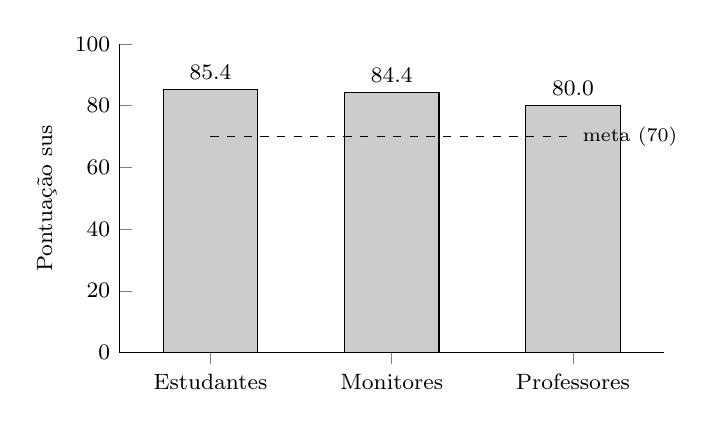
\begin{tikzpicture}
    \begin{axis}[
        ybar, bar width=12mm,
        width=0.7\textwidth, height=5.5cm,
        ymin=0, ymax=100, ylabel={Pontuação \acs{sus}},
        symbolic x coords={Estudantes, Monitores, Professores},
        xtick=data, enlarge x limits=0.25,
        nodes near coords,
        every node near coord/.append style={font=\footnotesize,
          /pgf/number format/fixed, /pgf/number format/fixed zerofill,
          /pgf/number format/precision=1},
        tick label style={font=\footnotesize}, label style={font=\footnotesize},
        axis x line*=bottom, axis y line*=left, clip=false,
      ]
      \addplot[fill=gray!40, draw=black] coordinates {
        (Estudantes,85.4) (Monitores,84.4) (Professores,80.0)
      };
      \draw[dashed] (axis cs:Estudantes,70) -- (axis cs:Professores,70)
        node[right, font=\scriptsize] {meta (70)};
    \end{axis}
  \end{tikzpicture}
  \fonte{Elaborado pelo próprio autor. Participaram 12 estudantes, 4
    monitores e 2 professores.}
\end{figure}

\begin{instrucao}
\orientacao{Pesquisas com pessoas}
Avaliações com usuários envolvem seres humanos e exigem cuidados éticos.
Converse com o orientador, antes de aplicar questionários ou entrevistas,
sobre a necessidade de submeter o projeto a um Comitê de Ética em Pesquisa.
Pesquisas de opinião com participantes não identificados podem ser
dispensadas desse registro, conforme a Resolução CNS nº 510/2016, mas a
decisão deve ser tomada caso a caso. Em qualquer situação, explique aos
participantes o objetivo da avaliação, obtenha o consentimento deles, não
colete dados pessoais desnecessários e apresente os resultados de forma
agregada. Coloque o roteiro de tarefas e o questionário em apêndice.
\end{instrucao}
